\documentclass[../lecture-notes.tex]{subfiles}

\begin{document}

\subsection{Quadratic Arithmetic Program}
\subsubsection{R1CS in Matrix Form}

While the Rank-1 Constraint System provides a powerful way to represent computations, it is not 
succinct at all, since the number of constraints depends linearly on the complexity of the problem 
being solved. In practical scenarios, this can require tens or even hundreds of thousands of 
constraints, sometimes even millions. The Quadratic Arithmetic Program (QAP) can address this issue.

\begin{remark}
    Understanding polynomials and their properties is crucial for this section. If you are not 
    confident in this area, it is better to revisit the corresponding chapter and refresh your
    knowledge. See \Cref{section:polynomials}.
\end{remark}

To define a constraint in the R1CS we need four vectors: three coefficient vectors ($\mathbf{a}$, $\mathbf{b}$, and
$\mathbf{c}$) and the witness one ($\mathbf{w}$). And that's just for one constraint. As you can imagine, many of
the values in these vectors are zeros. In circuits with thousands of inputs, outputs, and auxiliary
variables, where there are also thousands of constraints, you could end up with a millions of zeroes.
\begin{remark}
    A matrix in which most of the elements are zero in numerical analysis is usually called \textbf{sparse
    matrix}.
\end{remark}

So, we need to change the way how we manage coefficients and make the representation of such matrices and vectors succint (as required by the definition of SNARK).

\begin{theorem} 
    Consider a Rank-1 Constraint System (R1CS) defined by $m$ constraints. Each constraint is
    associated with coefficient vectors $\mathbf{a}_i$, $\mathbf{b}_i$, and $\mathbf{c}_i$, where $i \in \{1, 2, \dots, m\}$ and
    also a witness vector $\mathbf{w}$ consisting of $n$ elements.

    Then this system can also be represented using the corresponding matrices $A$, $B$, and $C$.
    \begin{align*}
        A = \begin{bmatrix}
            a_{11} & a_{12} & \dots & a_{1n} \\
            a_{21} & a_{22} & \dots & a_{2n} \\
            \vdots & \vdots & \ddots & \vdots \\
            a_{m1} & a_{m2} & \dots & a_{mn}
        \end{bmatrix} & \quad \\
        B = \begin{bmatrix}
            b_{11} & b_{12} & \dots & b_{1n} \\
            b_{21} & b_{22} & \dots & b_{2n} \\
            \vdots & \vdots & \ddots & \vdots \\
            b_{m1} & b_{m2} & \dots & b_{mn}
        \end{bmatrix} & \\
        C = \begin{bmatrix}
            c_{11} & c_{12} & \dots & c_{1n} \\
            c_{21} & c_{22} & \dots & c_{2n} \\
            \vdots & \vdots & \ddots & \vdots \\
            c_{m1} & c_{m2} & \dots & c_{mn}
        \end{bmatrix}
    \end{align*}

    such that all constraints can be reduced to the single equation:
    \begin{equation*}
        A\mathbf{w} \odot B\mathbf{w} = C\mathbf{w}
    \end{equation*}
    
    In this representation:
    \begin{itemize}
        \item Each $i$-th row of the matrices corresponds to the coefficients of a specific constraint.
        \item Each column of these matrices corresponds to the coefficients associated with a 
        particular element of the witness vector $\mathbf{w}$.
    \end{itemize}
\end{theorem}

\textbf{Proof.} Matrices defined this way can be expressed as
\begin{equation*}
    A = \begin{bmatrix}
        \mathbf{a}_1^{\top} \\ \mathbf{a}_2^{\top} \\ \vdots \\ \mathbf{a}_m^{\top}
    \end{bmatrix}, \quad B = \begin{bmatrix}
        \mathbf{b}_1^{\top} \\ \mathbf{b}_2^{\top} \\ \vdots \\ \mathbf{b}_m^{\top}
    \end{bmatrix}, \quad C = \begin{bmatrix}
        \mathbf{c}_1^{\top} \\ \mathbf{c}_2^{\top} \\ \vdots \\ \mathbf{c}_m^{\top}
    \end{bmatrix}
\end{equation*}

Consider an expression $A\mathbf{w}$:
\begin{equation*}
    A\mathbf{w} = \begin{bmatrix}
        \mathbf{a}_1^{\top} \\ \mathbf{a}_2^{\top} \\ \vdots \\ \mathbf{a}_m^{\top}
    \end{bmatrix}\begin{bmatrix}
        w_1 \\ w_2 \\ \vdots \\ w_n
    \end{bmatrix} = \begin{bmatrix}
        \mathbf{a}_1^{\top}\mathbf{w} \\ \mathbf{a}_2^{\top}\mathbf{w} \\ \vdots \\ \mathbf{a}_m^{\top}\mathbf{w}
    \end{bmatrix}
\end{equation*}

The last equality is a bit tricky to observe, so let us explain how we ended up with such expression. Notice that since $A \in \mathbb{F}^{m \times n}$ and $\mathbf{w} \in \mathbb{F}^n$, the product $A\mathbf{w}$ is a vector from $\mathbb{F}^m$. Now, for $j^{\text{th}}$ element of such vector, based on the matrix product definition, we have $(A\mathbf{w})_j = \sum_{\ell=1}^na_{j,\ell}w_{\ell}$ which is exactly an inner product between $\mathbf{a}_j$ and $\mathbf{w}$! Therefore, we have:
\begin{equation*}
    A\mathbf{w} = \begin{bmatrix}
        \langle \mathbf{a}_1, \mathbf{w}\rangle \\
        \langle \mathbf{a}_2, \mathbf{w}\rangle \\
        \vdots \\
        \langle \mathbf{a}_m, \mathbf{w}\rangle 
    \end{bmatrix}, \quad \\
    B\mathbf{w} = \begin{bmatrix}
        \langle \mathbf{b}_1, \mathbf{w}\rangle \\
        \langle \mathbf{b}_2, \mathbf{w}\rangle \\
        \vdots \\
        \langle \mathbf{b}_m, \mathbf{w}\rangle 
    \end{bmatrix}, \quad \\
    C\mathbf{w} = \begin{bmatrix}
        \langle \mathbf{c}_1, \mathbf{w}\rangle \\
        \langle \mathbf{c}_2, \mathbf{w}\rangle \\
        \vdots \\
        \langle \mathbf{c}_m, \mathbf{w}\rangle 
    \end{bmatrix}
\end{equation*}

Therefore, $A\mathbf{w} \odot B\mathbf{w} = C\mathbf{w}$ is equivalent to the system of $m$ constraints:
\begin{equation*}
    \langle \mathbf{a}_j, \mathbf{w}\rangle \times \langle \mathbf{b}_j, \mathbf{w} \rangle = \langle \mathbf{c}_j, \mathbf{w} \rangle, \; j \in \{1,\dots,m\}.
\end{equation*}

\begin{example}
    The vectors $\mathbf{a}_i$ from the previous examples have the form:
    \begin{align*}
        \mathbf{a}_1 &= (0, 0, 1, 0, 0, 0, 0) \\
        \mathbf{a}_2 &= (0, 0, 0, 1, 0, 0, 0) \\
        \mathbf{a}_3 &= (0, 0, 1, 0, 0, 0, 0) \\
        \mathbf{a}_4 &= (1, 0, -1, 0, 0, 0, 0)
    \end{align*}
    This corresponds to $n = 7, m = 4$
    \begin{equation*}
        \begin{aligned}            
        &A = \begin{bmatrix}
            a_{1,1} & a_{1,2} & a_{1,3} & a_{1,4} & a_{1,5} & a_{1,6} & a_{1,7} \\
            a_{2,1} & a_{2,2} & a_{2,3} & a_{2,4} & a_{2,5} & a_{2,6} & a_{2,7} \\
            a_{3,1} & a_{3,2} & a_{3,3} & a_{3,4} & a_{3,5} & a_{3,6} & a_{3,7} \\
            a_{4,1} & a_{4,2} & a_{4,3} & a_{4,4} & a_{4,5} & a_{4,6} & a_{4,7}
        \end{bmatrix} = \\ &\text{\;\;\,} = \begin{bmatrix}
            0 & 0 & 1 & 0 & 0 & 0 & 0 \\
            0 & 0 & 0 & 1 & 0 & 0 & 0 \\
            0 & 0 & 1 & 0 & 0 & 0 & 0 \\
            1 & 0 & -1 & 0 & 0 & 0 & 0 
        \end{bmatrix}
    \end{aligned}
\end{equation*}
\end{example}

\subsubsection{Polynomial Interpolation}

OK, now is the time to define how we are going to build polynomials! Notice that the columns of these matrices (say, column $(a_{1,i},a_{2,i},a_{3,i},a_{4,i})$ in matrix $A$ from example above) represent the mappings from constraint number $i$ to the corresponding
coefficient of the $j$ element in the witness vector!

\begin{example}
    Consider the witness from the previous examples: 
    \begin{equation*}
        \mathbf{w} = (1, r, x_1, x_2, x_3, \mathsf{mult}, \mathsf{selectMult})
    \end{equation*}
    For element $x_1$ we are interested in the third columns of the $A$, $B$ and $C$ matrices, as
    it's placed on the third position in the witness vector, so $j = 3$.\\
    For matrix $A$:
    \begin{center}
        \begin{tikzpicture}
            % Node to contain the pmatrix
            \node (A) at (0,0) {$
                \begin{bmatrix}
                    0 & 0 & \textcolor{red!100}{1} & 0 & 0 & 0 & 0 \\
                    0 & 0 & \textcolor{red!100}{0} & 1 & 0 & 0 & 0 \\
                    0 & 0 & \textcolor{red!100}{1} & 0 & 0 & 0 & 0 \\
                    1 & 0 & \textcolor{red!100}{-1} & 0 & 0 & 0 & 0 \\
                \end{bmatrix}
            $};
        
        \end{tikzpicture}
    \end{center}

    Thus, for constraint number 4 ($i = 4$) the coefficient of $x_1$ is $-1$:
    \begin{center}
        \begin{tikzpicture}
            % Node to contain the pmatrix
            \node (A) at (0,0) {$
                \begin{bmatrix}
                    0 & 0 & \textcolor{red!100}{1} & 0 & 0 & 0 & 0 \\
                    0 & 0 & \textcolor{red!100}{0} & 1 & 0 & 0 & 0 \\
                    0 & 0 & \textcolor{red!100}{1} & 0 & 0 & 0 & 0 \\
                    \textcolor{blue!100}{1} & \textcolor{blue!100}{0} & \textcolor{black!100}{-1} & \textcolor{blue!100}{0} & \textcolor{blue!100}{0} & \textcolor{blue!100}{0} & \textcolor{blue!100}{0} \\
                \end{bmatrix}
            $};
        
        \end{tikzpicture}
    \end{center}
\end{example}

Good, so now we know that for the $j$th element in the witness vector there are $m$ (the number of constraints) corresponding values in matrices $A$, $B$, and $C$. Now, we want to encode this statement in a form of a polynomial. 
As we know from the previous chapters, such a mapping in math can be built using the Lagrange polynomial interpolation.

\begin{remark}
    As a remainder, the Lagrange interpolation polynomial for a given set of points 
    $\{(x_0,y_0),(x_1,y_1),\dots,(x_n,y_n)\} \subset \mathbb{F} \times \mathbb{F}$
    can be built with the following formula:
    \begin{equation*}
        L(x) = \sum_{i=0}^{n} y_i \ell_i(x), \quad \ell_i(x) = \prod_{j=0, j \neq i}^{n} \frac{x-x_j}{x_i-x_j}.
    \end{equation*}  
\end{remark}

For a given column $j \in \{1, 2, \dots, n\}$ in a matrix $A$ the set of points that define the
variable polynomial $A_j(x)$ can be defined as $\{(i, a_{ij}): i \in \{1, 2, \dots, m\}\}$. In other words,
we want to interpolate $n$ polynomials $A_j \in \mathbb{F}[X]$ such that:
\begin{equation*}
    A_j(i) = a_{i,j}, \; i \in \{1,2,\dots,m\}, \; j \in \{1,2,\dots,n\}
\end{equation*}

The same is true for matrices $B$ and $C$, resulting in $3n$ polynomials, $n$ for each of the
coefficients matrices:
\begin{align*}
    &A_1(x), A_2(x), \dots, A_n(x), \\
    &B_1(x), B_2(x), \dots, B_n(x), \\
    &C_1(x), C_2(x), \dots, C_n(x)
\end{align*}

\begin{example}
    Considering the witness vector $\mathbf{w}$ and matrix $A$ from the previous example, for the variable
    $x_1$, the next set of points can be derived:
    \begin{equation*}
        \{(1,1), (2,0), (3,1), (4,-1)\}
    \end{equation*}
    We can see that it is used in the 1st, 3rd, and 4th constraints as the values of the coefficients
    are not zero.
    
    The Lagrange interpolation polynomial for this set of points can be built as follows (for the demonstration purposes, assume we are working in the field $\mathbb{R}$):
    \begin{align*}
        \ell_1(x) &= -\frac{(x - 2)(x - 3)(x - 4)}{6}, \\
        \ell_2(x) &= \frac{(x - 1)(x - 3)(x - 4)}{2},  \\
        \ell_3(x) &= -\frac{(x - 1)(x - 2)(x - 4)}{2}, \\
        \ell_4(x) &= \frac{(x - 1)(x - 2)(x - 3)}{6}.
    \end{align*}

    Thus, the polynomial is given by:
    \begin{equation*}    
        \begin{aligned}
            A_1(x) &= 1 \cdot \ell_1(x) + 0 \cdot \ell_2(x) + 1 \cdot \ell_3(x) + (-1) \cdot \ell_4(x) \\
            &= -\frac{5}{6}x^3 + 6x^2 - \frac{79}{6}x + 9.
        \end{aligned}
    \end{equation*}
Therefore, the final Lagrange interpolation polynomial is:
    \begin{equation*}
        A_1(x) = -\frac{5}{6}x^3 + 6x^2 - \frac{79}{6}x + 9
    \end{equation*}

    As shown in Illustration below, the curve intersects all the given points.
    In this figure, the x-axis represents the constraint number, and the y-axis represents the 
    coefficients of the $x_1$ witness element.

    \begin{center}
        \scalebox{0.8}{
        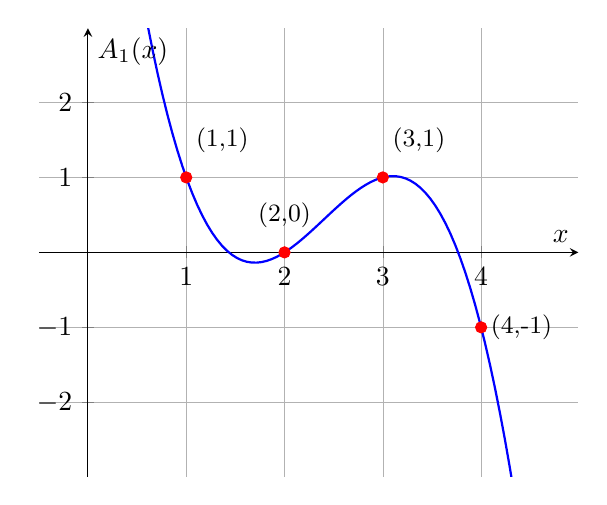
\begin{tikzpicture}
            \begin{axis}[
                axis lines = middle,
                xlabel = {$x$},
                ylabel = {$A_1(x)$},
                ymin = -2.99, ymax = 2.99,
                xmin = -0.5, xmax = 4.99,
                domain = 0:5,
                samples = 100,
                ytick = {-3,...,3},
                xtick = {0,1,...,5},
                grid = both, 
                grid style = {line width=.1pt, draw=gray!20},
                major grid style = {line width=.2pt, draw=gray!60}
            ]
            \addplot[
                color=blue,
                thick
            ]
            {-5/6*x^3 + 6*x^2 - 79/6*x + 9};
            \addplot[
                only marks,
                mark=*,
                color=red
            ]
            coordinates {(1,1) (2,0) (3,1) (4,-1)};
    
            \node at (axis cs:1,1.5) [anchor=west] {\small (1,1)};
            \node at (axis cs:2,0.2) [anchor=south] {\small (2,0)};
            \node at (axis cs:3,1.5) [anchor=west] {\small (3,1)};
            \node at (axis cs:4,-1) [anchor=west] {\small (4,-1)};
            
            \end{axis}
        \end{tikzpicture}
        }

        \scriptsize\textbf{Illustration:} The Lagrange inteprolation polynomial for points $\{(1,1), (2,0), (3,1), (4,-1)\}$ visualized over $\mathbb{R}$.
    \end{center}
\end{example}

\begin{remark}
    One might a reasonable question: why do we choose $x$-coordinates to be the indeces of the corresponding constraints? 
    Actually, just for convenience purposes. We could have assigned any \textit{unique} index from $\mathbb{F}$ to each 
    constraint (say, $t_i$ for each $i \in \{1,\dots,m\}$) and interpolate through these points:
    \begin{equation*}
        A_j(t_i) = a_{i,j}, \; i \in \{1,2,\dots,m\}, \; j \in \{1,2,\dots,n\}
    \end{equation*}

    As we will see in the subsequent lectures, we can define the $x$-coordinates in much more clever way to reduce the workload
    needed for interpolation. But for now, we will stick to this simple version.
\end{remark}

\begin{remark}
    The degree of the coefficient polynomials does not exceed $m - 1$, which follows from the Lagrange interpolation properties.
\end{remark}

\subsubsection{Putting All Together!}

Now, using coefficients encoded with polynomials, a constraint number $X \in \{1, \dots\ m\}$, from
a constraint system with a witness vector $\mathbf{w}$ can be built in the next way:
\begin{align*}
    &(w_1A_1(X) + w_2A_2(X) + \dots + w_nA_n(X)) \times \\ &\times (w_1B_1(X) + w_2B_2(X) + \dots + w_nB_n(X)) = \\ &= (w_1C_1(X) + w_2C_2(X) + \dots + w_nC_n(X))
\end{align*}

Or, written more concisely:
\begin{equation*}
    \left( \sum_{i = 1}^{n} w_iA_i(X) \right) \times \left( \sum_{i = 1}^{n} w_iB_i(X) \right) = \left( \sum_{i = 1}^{n} w_iC_i(X) \right)
\end{equation*}

\begin{remark}
    Hold on, but why does it hold? Let us substitute any $X=j$ into this equation:
    \begin{equation*}
        \left( \sum_{i = 1}^{n} w_iA_i(j) \right) \times \left( \sum_{i = 1}^{n} w_iB_i(j) \right) = \left( \sum_{i = 1}^{n} w_iC_i(j) \right)
    \end{equation*}

    Recall that we interpolated polynomials to have $A_i(j) = a_{j,i}$. Therefore, the equation above can be reduced to:
    \begin{equation*}
        \left( \sum_{i = 1}^{n} w_ia_{j,i} \right) \times \left( \sum_{i = 1}^{n} w_ib_{j,i} \right) = \left( \sum_{i = 1}^{n} w_ic_{j,i} \right)
    \end{equation*}

    But hold on again! Notice that $\sum_{i = 1}^{n} w_ia_{j,i} = \langle \mathbf{w}, \mathbf{a}_j \rangle$ and therefore we have:
    \begin{equation*}
        \langle \mathbf{w}, \mathbf{a}_j \rangle \times \langle \mathbf{w}, \mathbf{b}_j \rangle = \langle \mathbf{w}, \mathbf{c}_j \rangle \; \forall j \in \{1,\dots,m\},
    \end{equation*}
    
    so we ended up with the initial $m$ constraint equations!
\end{remark}

Now let us define polynomials $A(X)$, $B(X)$, $C(X)$ for easier notation: 
\begin{equation*}
    \begin{aligned}
        A(X) = \sum_{i = 1}^{n} w_iA_i(X), \\ \quad B(X) = \sum_{i = 1}^{n} w_iB_i(X), \\ \quad C(X) = \sum_{i = 1}^{n} w_iC_i(X)        
    \end{aligned}
\end{equation*}

Therefore, our constraint can be rewritten as $A + B = C$ --- much less scary-looking than what we have written before. OK, but what does it give us? 

Notice that if $A(X) \times B(X)=C(X) \forall j \in \{1,\dots,m\}$ then polynomial, defined as $M(X) := A(X) \times B(X)-C(X)$, has zeros at all elements from the set $\Omega = \{1,\dots,m\}$. Define the so-called \textbf{vanishing polynomial} on $\Omega$ as:
\begin{equation*}
    Z_{\Omega}(X) := \prod_{\omega \in \Omega} (X - \omega) = \prod_{i=1}^m (X - i)
\end{equation*} 

Now, if $M(X)$ vanishes on all points from $\Omega$, it means that $Z_{\Omega}$ must divide $M$, so $Z_{\Omega} \mid M$. But that means
that $M$ can be divided by $Z_{\Omega}$ without remainder! In other words, there exists some polynomial $H$ such that $M=Z_{\Omega}H$. We further drop index $\Omega$ for simplicity. 

All in all, let us give the definition of a \textbf{Quadratic Arithmetic Program}.

\begin{definition}[Quadratic Arithmetic Program]
    Suppose that $m$ R1CS constraints with a witness of size $n$ are written in a form
    \begin{equation*}
        A\mathbf{w} \odot B\mathbf{w} = C\mathbf{w}, \; A,B,C \in \mathbb{F}^{m \times n}
    \end{equation*}

    Then, the \textbf{Quadratic Arithmetic Program} consists of $3n$ polynomials $A_1,\dots,A_n$, $B_1,\dots,B_n$, $C_1,\dots,C_n$ such that:
    \begin{equation*}
        \begin{aligned}
            &\forall i \in \{1,\dots,m\} \; \forall j \in \{1,\dots,n\}: \\
            &A_j(i) = a_{i,j}, \; B_j(i) = b_{i,j}, \; C_j(i) = c_{i,j}            
        \end{aligned}
    \end{equation*}

    Then, $\mathbf{w} \in \mathbb{F}^n$ is a valid assignment for the given QAP and \textbf{target polynomial} $Z(X) = \prod_{i=1}^m (X-i)$ if and only if there exists such a polynomial $H(X)$ such that
    \begin{equation*}
        \begin{aligned}
            &\left( \sum_{i = 1}^{n} w_iA_i(X) \right)\left( \sum_{i = 1}^{n} w_iB_i(X) \right) - \left( \sum_{i = 1}^{n} w_iC_i(X) \right) = \\ &= Z(X)H(X)            
        \end{aligned}
    \end{equation*}
\end{definition}

This was our final step in representing a high-level programming language to some math primitive.
We have managed to encode our computation to a single polynomial!

\subsubsection*{Remark on operations between polynomials}

\begin{remark}
    Some pretty obvious property should be noted. In the theorem ~\ref{thm:polynomials-degree-op}
    it was said about the degree of polynomials after their multiplication or addition, but what
    about their values?

    Let $p(x), q(x) \in \mathbb{F}[x]$ be two polynomials over a field $\mathbb{F}$. Define the 
    polynomial $r(x)$ as the sum of $p(x)$ and $q(x)$:
    \begin{equation*}
        r(x) = p(x) + q(x)
    \end{equation*}
    Then, for any point $x \in \mathbb{F}$, the value of $r(x)$ is equal to the sum of the
    values of $p(x)$ and $q(x)$ at that point. Therefore, the set of points corresponding to the 
    polynomial $r(x)$ is given by:
    \begin{equation*}
        \{(x, y) \in \mathbb{F} \times \mathbb{F} \mid x \in \mathbb{F}, \, y = p(x) + q(x) \}
    \end{equation*}

    The same is true for product.
\end{remark}

\begin{example}
    Consider two polynomials $p(x)$ and $q(x)$ defined over the real numbers $\mathbb{R}$:
    \begin{equation*}
        p(x) = -\frac{1}{2}x^2 + \frac{3}{2}x, \quad
        q(x) = \frac{1}{3}x^3 - 2x^2 + \frac{8}{3}x + 1.
    \end{equation*}
    The sets of points $\{(0, 0), (1, 1), (2, 1), (3, 0)\}$ and $\{(0, 1), (1, 2), (2, 1), (3, 0)\}$
    lie on the graphs of $p(x)$ and $q(x)$, respectively.\\
    
    The sum of these polynomials can be calculated as:
    \begin{align*}
        r(x) &= (-\frac{1}{2}x^2 + \frac{3}{2}x) + (\frac{1}{3}x^3 - 2x^2 + \frac{8}{3}x + 1) \\
             &= \frac{1}{3}x^3 - 2\frac{1}{2}x^2 + 4\frac{1}{6}x + 1
    \end{align*}
    The resulting polynomial $r(x)$ corresponds to the set of points $\{(0, 1), (1, 3), (2, 2), (3, 0)\}$.
    
    As you can see (Figure~\ref{fig:example-polynomial-addition}), the values at each point for the 
    corresponding $x$ are the sum of the initial polynomials' points.
\end{example}

\begin{figure}[H]
    \centering
    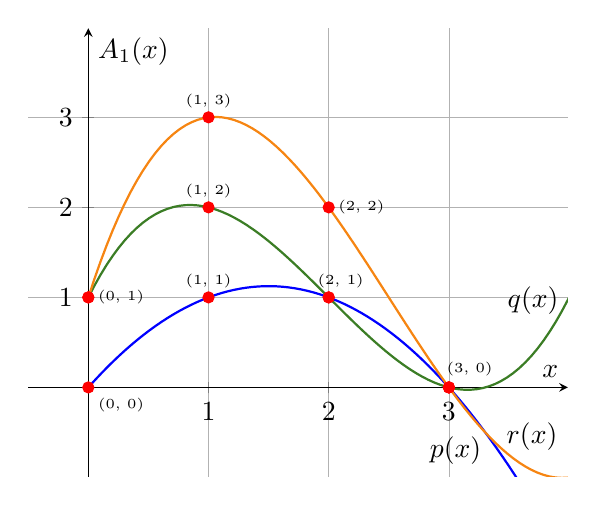
\begin{tikzpicture}
        \begin{axis}[
            axis lines = middle,
            xlabel = {$x$},
            ylabel = {$A_1(x)$},
            ymin = -0.99, ymax = 3.99,
            xmin = -0.5, xmax = 3.99,
            domain = 0:5,
            samples = 100,
            ytick = {-1,...,4},
            xtick = {0,1,...,4},
            grid = both,
            grid style = {line width=.1pt, draw=gray!20},
            major grid style = {line width=.2pt, draw=gray!60}
        ]

        % p(x)
        \addplot[
            color=blue,
            thick
        ]
        {3/2*x - 1/2*x^2};
        \addplot[
            only marks,
            mark=*,
            color=red
        ]
        coordinates {(0, 0) (1, 1) (2, 1) (3, 0)};
        \node at (axis cs:3.35,-0.7) [anchor=east] {\text{$p(x)$}};

        \node at (axis cs:0,-0.2) [anchor=west] {\tiny (0, 0)};
        \node at (axis cs:1,1) [anchor=south] {\tiny (1, 1)};
        \node at (axis cs:2.1,1) [anchor=south] {\tiny (2, 1)};
        \node at (axis cs:2.9,0.2) [anchor=west] {\tiny (3, 0)};
            
        % q(x)
        \addplot[
            color=OliveGreen,
            thick
        ]
        {1/3*x^3 - 2*x^2 + 8/3*x + 1};
        \addplot[
            only marks,
            mark=*,
            color=red
        ]
        coordinates {(0,1) (1,2) (2,1) (3, 0)};
        \node at (axis cs:3.7,0.7) [anchor=south] {\text{$q(x)$}};

        \node at (axis cs:0,1) [anchor=west] {\tiny (0, 1)};
        \node at (axis cs:1,2) [anchor=south] {\tiny (1, 2)};

        % r(x)
        \addplot[
            color=BurntOrange,
            thick
        ]
        {1/3*x^3 - 5/2*x^2 + 25/6*x + 1};
        \addplot[
            only marks,
            mark=*,
            color=red
        ]
        coordinates {(0,1) (1,3) (2,2) (3, 0)};
        \node at (axis cs:3.4,-0.55) [anchor=west] {\text{$r(x)$}};

        \node at (axis cs:1,3) [anchor=south] {\tiny (1, 3)};
        \node at (axis cs:2,2) [anchor=west] {\tiny (2, 2)};

        \end{axis}
    \end{tikzpicture}
    \caption{Addition of two polynomials}
    \label{fig:example-polynomial-addition}
\end{figure}

\subsection{Probabilistically Checkable Proofs}

Before going further we should get acquainted with one more concept from the computational 
complexity theory, that have an important application in zk-SNARK and provides the theoretical 
backbone. 

A Probabilistically Checkable Proof (PCP) is a type of proof system where the verifier can 
efficiently check the correctness of a proof by examining only a small, random portion of it, rather
than verifying it entirely. 
\begin{definition}
    A language $\mathcal{L} \subseteq \Sigma^*$ (for some given alphabet $\Sigma$) is in the class $\mathsf{PCP}(r,q)$ (\textbf{probabilistically checkable proofs}), 
    where $r$ is the \emph{randomness complexity} and $q$ is the \emph{query complexity}, 
    if for a given pair of algorithms $(\mathcal{P}, \mathcal{V})$: 
    \begin{itemize}
        \item \emph{Syntax:} $\mathcal{P}$ calculates a proof (bit string) $\pi \in \Sigma^*$ in polynomial time $\mathsf{poly}(|x|)$ of the common input $x$. The prover $\mathcal{P}$ and verifier $\mathcal{V}$ interact, where the verifier has an oracle access to $\pi$ (meaning, he queries it at any position).
        \item \emph{Complexity:} $\mathcal{V}$ uses at most $r$ random bits to decide which part of the proof to 
        query and the verifier queries at most $q$ bits of the proof.
    \end{itemize}
    
    Such pair of algorithms $(\mathcal{P}, \mathcal{V})$ should satisfy the following properties (with a security parameter $\lambda \in \mathbb{N}$):
    \begin{itemize}
        \item \textbf{Completeness}: If $x \in \mathcal{L}$, then $\Pr[\mathcal{V}^{\pi}(x) = 1] = 1$.
        \item \textbf{Soundness}: If $x \notin \mathcal{L}$, then for any possible (malicious) proof $\pi^*$, 
        \begin{equation*}
            \Pr[\mathcal{V}^{\pi^*}(x) = 1] = \mathsf{negl}(\lambda).
        \end{equation*}
    \end{itemize}
\end{definition}
This allows a verification of huge statements with high confidence while using limited computational
resources. See \Cref{fig:pcp}.

\begin{theorem}{\textbf{PCP theorem (PCP characterization theorem)}\\}
    Any decision problem in $\mathsf{NP}$ has a PCP verifier that uses logarithmic randomness 
    $O(\log n)$ and a constant number of queries $O(1)$, independent of $n$.
    \begin{equation*}
        \mathsf{NP} = \mathsf{PCP}(O(\log n), O(1))
    \end{equation*}
\end{theorem}

\begin{figure}[H]
    \centering
    \scalebox{0.7}{
    \begin{tikzpicture}
        \node[inner sep=0pt, align=center] at (-4.0, 0.0) (prover) {
\includegraphics[width=1.25cm]{lectures/images/common/prover.png}\\Prover $\mathcal{P}$};
        \node[inner sep=0pt, align=center] at (4.0, 0.0) (verifier) {
\includegraphics[width=1.25cm]{lectures/images/common/verifier.png}\\Verifier $\mathcal{V}$};

        \draw[fill=gray!20!white, ultra thick] (-2.0, 4) rectangle (2.0, 3.25);

        % Query boxes
        \draw[fill=blue!60!white, ultra thick] (-1.0, 4) rectangle (-0.8, 3.25);
        \node at (-0.9, 4.35) (pcp) {$q_1$};
        \draw[fill=blue!60!white, ultra thick] (0.0, 4) rectangle (0.2, 3.25);
        \node at (0.1, 4.35) (pcp) {$q_2$};
        \draw[fill=blue!60!white, ultra thick] (0.5, 4) rectangle (0.7, 3.25);
        \node at (0.6, 4.35) (pcp) {$q_3$};
        \node at (0, 2.85) (pcp) {\textbf{PCP Oracle}};

        \draw[-{Stealth[length=3mm]},line width=0.4mm] (prover)--(pcp) node[midway, left=3mm]{Generate an oracle ($\pi$)};
        \draw[-{Stealth[length=3mm]},line width=0.4mm] (verifier)--(pcp) node[midway, right=3mm]{Point queries $q_1,\dots,q_m$};
    \end{tikzpicture}
    }
    \caption{Illustration of a Probabilistically Checkable Proof (PCP) system. The prover $\mathcal{P}$ generates a PCP oracle $\pi$ that is queried by the verifier $\mathcal{V}$ at specific points $q_1,\dots,q_m$.}
    \label{fig:pcp}
\end{figure}

However, despite the fact that PCP is a very powerful tool, it is not used directly in zk-SNARKs. We need to extend it a bit to make it more suitable for our purposes.

Three main extensions of PCPs that are frequently used in SNARKs are:
\begin{itemize}
    \item \textbf{IPCP} (\textbf{Interactive PCP}): The prover commits to the PCP oracle and then, based on the interaction between the prover and verifier, the verifier queries the oracle and decides whether to accept the proof.
    \item \textbf{IOP} (\textbf{Interactive Oracle Proof}): The prover and verifier interact and on each round, the prover commits to a new oracle. The verifier queries the oracle and decides whether to accept the proof.
    \item \textbf{LPCP} (\textbf{Linear PCP}): The prover commits to a linear function and the verifier queries the function at specific points.
\end{itemize}

\begin{figure}[H]
    \centering
    \scalebox{0.5}{
    \begin{tikzpicture}
        \node[inner sep=0pt, align=center] at (-4.0, 0.0) (prover) {
\includegraphics[width=1.25cm]{lectures/images/common/prover.png}\\Prover $\mathcal{P}$};
        \node[inner sep=0pt, align=center] at (4.0, 0.0) (verifier) {
\includegraphics[width=1.25cm]{lectures/images/common/verifier.png}\\Verifier $\mathcal{V}$};

        % Oracle 1
        \node at (-2.0, 5.625) (oracle_1_left) {};
        \node at (2.0, 5.625) (oracle_1_right) {};
        \draw[fill=gray!20!white, ultra thick] (-2.0, 6) rectangle (2.0, 5.25);
        \draw[fill=blue!60!white, ultra thick] (-1.0, 6) rectangle (-0.8, 5.25);
        \node at (-0.9, 6.35) (pcp) {$q_1$};
        \draw[fill=blue!60!white, ultra thick] (0.0, 6) rectangle (0.2, 5.25);
        \node at (0.1, 6.35) (pcp) {$q_2$};
        \draw[fill=blue!60!white, ultra thick] (0.5, 6) rectangle (0.7, 5.25);
        \node at (0.6, 6.35) (pcp) {$q_3$};
        \node at (0, 4.85) (pcp) {\textbf{PCP Oracle \#1}};

        % Oracle 2
        \node at (-2.0, 3.625) (oracle_2_left) {};
        \node at (2.0, 3.625) (oracle_2_right) {};
        \draw[fill=gray!20!white, ultra thick] (-2.0, 4) rectangle (2.0, 3.25);
        \draw[fill=blue!60!white, ultra thick] (-0.4, 4) rectangle (-0.2, 3.25);
        \node at (-0.3, 4.35) (pcp) {$q_1'$};
        \draw[fill=blue!60!white, ultra thick] (0.2, 4) rectangle (0.4, 3.25);
        \node at (0.3, 4.35) (pcp) {$q_2'$};
        \draw[fill=blue!60!white, ultra thick] (1.5, 4) rectangle (1.7, 3.25);
        \node at (1.6, 4.35) (pcp) {$q_3'$};
        \node at (0, 2.85) (pcp) {\textbf{PCP Oracle \#2}};

        % Oracle 3
        \node at (-2.0, 1.625) (oracle_3_left) {};
        \node at (2.0, 1.625) (oracle_3_right) {};
        \draw[fill=gray!20!white, ultra thick] (-2.0, 2) rectangle (2.0, 1.25);
        \draw[fill=blue!60!white, ultra thick] (-1.5, 2) rectangle (-1.3, 1.25);
        \node at (-1.4, 2.35) (pcp) {$q_1''$};
        \draw[fill=blue!60!white, ultra thick] (0.3, 2) rectangle (0.5, 1.25);
        \node at (0.4, 2.35) (pcp) {$q_2''$};
        \draw[fill=blue!60!white, ultra thick] (1.0, 2) rectangle (1.2, 1.25);
        \node at (1.1, 2.35) (pcp) {$q_3''$};
        \node at (0, 0.85) (pcp) {\textbf{PCP Oracle \#3}};

        \draw[-{Stealth[length=3mm]},line width=0.4mm] (prover)--(oracle_1_left) node[midway, left=3mm]{Commit to oracles ($\pi_1,\dots,\pi_r$)};
        \draw[-{Stealth[length=3mm]},line width=0.4mm] (verifier)--(oracle_1_right) node[midway, right=3mm]{Point queries ($\mathbf{q}_1,\dots,\mathbf{q}_r$)};
        \draw[-{Stealth[length=3mm]},line width=0.4mm] (prover)--(oracle_2_left) node[midway, left=3mm]{};
        \draw[-{Stealth[length=3mm]},line width=0.4mm] (verifier)--(oracle_2_right) node[midway, right=3mm]{};
        \draw[-{Stealth[length=3mm]},line width=0.4mm] (prover)--(oracle_3_left) node[midway, left=3mm]{};        
        \draw[-{Stealth[length=3mm]},line width=0.4mm] (verifier)--(oracle_3_right) node[midway, right=3mm]{};

        % Two arrows to left and to right between the prover and verifier with the "Interaction" label
        \draw[{Stealth[length=3mm]}-{Stealth[length=3mm]},line width=0.4mm,dashed] (prover) to node[midway, below]{Interaction} (verifier);
    \end{tikzpicture}
    }
    \caption{Illustration of an Interactive Oracle Proof (IOP). On each round $i$ ($1 \leq i \leq r$), $\mathcal{V}$ sends a message $m_i$, and $\mathcal{P}$ commits to a new oracle $\pi_i$, which $\mathcal{V}$ can query at $\mathbf{q}_i=(q_{i,1},\dots,q_{i,m})$.}
    \label{fig:pcp}
\end{figure}

While IOPs will be later used for PLONK and zk-STARKs, we will focus on Linear PCPs in the context of Groth16 zk-SNARK. Let us define it below.

\begin{definition}[Linear PCP]
    A \textbf{Linear PCP} is a PCP where the prover commits to a linear function $\boldsymbol{\pi} = (\pi_1,\dots,\pi_k)$ and the verifier queries the function at specific points $\boldsymbol{q}_1,\dots,\boldsymbol{q}_r$. Then, the prover responds with the values of the function at these points:
    \begin{equation*}
        \langle \boldsymbol{\pi}_1, \mathbf{q}_1 \rangle, \langle \boldsymbol{\pi}_2, \mathbf{q}_2 \rangle, \dots, \langle \boldsymbol{\pi}_r, \mathbf{q}_r \rangle.
    \end{equation*}
\end{definition}

\begin{example}[QAP as a Linear PCP]
    Recall that key QAP equation is:
    \begin{equation*}
        \begin{aligned}
            &\left(\sum_{i=1}^nw_iL_i(x)\right)\left(\sum_{i=1}^nw_iR_i(x)\right) - \left(\sum_{i=1}^nw_iO_i(x)\right) = \\ &= Z(x)H(x).            
        \end{aligned}
    \end{equation*}

    Now, the notation might be confusing, but firstly, we denote vectors of polynomials: 
    \begin{align*}
        \boldsymbol{L}(x) & = (L_1(x),\dots,L_n(x)), \\
        \boldsymbol{R}(x) & = (R_1(x),\dots,R_n(x)), \\
        \boldsymbol{O}(x) & = (O_1(x),\dots,O_n(x)).
    \end{align*}
    
    Now, consider the following \textbf{linear PCP for QAP}:
    \begin{enumerate}
        \item $\mathcal{P}$ commits to an extended witness $\mathbf{w}$ and coefficients $\mathbf{h} = (h_1,\dots,h_n)$ of $H(x)$.
        \item $\mathcal{V}$ samples $\gamma \xleftarrow{R} \mathbb{F}$ and sends query $\boldsymbol{\gamma} = (\gamma,\gamma^2,\dots,\gamma^n)$ to $\mathcal{P}$.
        \item $\mathcal{P}$ reveals the following values:
        \begin{equation*}
            \begin{aligned}
                &\pi_1 \gets \langle \mathbf{w}, \boldsymbol{L}(\gamma) \rangle, \quad \pi_2 \gets \langle \mathbf{w}, \boldsymbol{R}(\gamma) \rangle, \quad \\ & \pi_3 \gets \langle \mathbf{w}, \boldsymbol{O}(\gamma) \rangle, \quad \pi_4 \gets Z(\gamma) \cdot \langle \mathbf{h}, \boldsymbol{\gamma} \rangle.                
            \end{aligned}
        \end{equation*}
        \item $\mathcal{V}$ checks whether $\pi_1\pi_2 - \pi_3 = \pi_4$.
    \end{enumerate}
\end{example}

Of course, the above example cannot be used as it is: at the very least, we have not specified how the prover commits to the extended witness $\mathbf{w}$ and coefficients $\mathbf{h}$ and then ensures consistency of $\pi_1,\dots,\pi_4$ with these commitments. For that reason, we need some more tools to make it work which we learned in the previous lectures.

\subsection{QAP as a Linear PCP}

When constructing a Quadratic Arithmetic Program (QAP) for a circuit $\Circ$, we represented the whole circuit's 
computation using the following relation:
\begin{equation*}
    L(x)R(x) - O(x) = Z(x)H(x),
\end{equation*}
where by $L(x)$, $R(x)$, $O(x)$ we denote the polynomials that represent the left, right and output 
wires of the circuit, respectively. $Z(x)$ is the target polynomial, while
$H(x) := M(x)\big/Z(x)$ for master polynomial $M(x) = L(x)R(x) - O(x)$ is the quotient polynomial.

We effectively managed to transform all the circuit's constraints, and computations in the short form.
It still allows one to verify that each computational step is preserved by verifying the 
polynomial evaluation in specific (random) points, instead of recomputing everything. However, it is 
not quite clear why such a check is safe and how it can be used in a PCP. In other words, why checking that $L(s)R(s)-O(s)=Z(s)H(s)$ for randomly selected $s$ is enough to verify the circuit $\Circ$?

\textbf{Soundness justification.} Why is it safe to use such a check? As it was said early, 
we perform all the computations in some finite field $\mathbb{F}$. The 
polynomials $L(x)$, $R(x)$ and $O(x)$ are interpolated polynomials using $\left| \Circ \right|$ (number of gates) points, so 
\begin{equation*}
    \deg(L) \le \left| \Circ \right|, \quad 
    \deg(R) \le \left| \Circ \right|, \quad 
    \deg(O) \le \left| \Circ \right|
\end{equation*}

Thus, using properties of polynomials' degrees, we can estimate the degree of polynomial $M(x) = L(x)R(x) - O(x)$.
\begin{equation*}
    \deg(M) \leq \max\{\deg(L) + \deg(R), \deg(O)\} \leq 2 \left| \Circ \right|
\end{equation*}

Now, using the Schwartz-Zippel \Cref{lemma:sz},
we can deduce that if an adversary $\mathcal{A}$ does not know a valid witness $\mathbf{w}$, 
resolving the circuit $\Circ$, he can compute a polynomial $\widetilde{M}(x) \gets \mathcal{A}(\cdot)$ that 
satisfies a verifier $\mathcal{V}$ with probability less than $2 \left| \Circ \right|/|\mathbb{F}|$. To put it formally, we can write:
\begin{equation*}
    \mathop{\text{Pr}}_{s \xleftarrow{R} \mathbb{F}}[\widetilde{M}(s) = M(s)] \leq \frac{2 \left| \Circ \right|}{|\mathbb{F}|}
\end{equation*}
This probability becomes negligible as $|\mathbb{F}|$ grows large, which is typically the case, giving us soundness. In the same time, the
verifier accepts the $M(x)$ generated using a valid witness with probability $1$ giving us the 
completeness, so, we can categorize QAP as PCP. 

We will modify the form of our proof with the next modifications, but still preserve the PCP 
properties.

In the following sections, we will introduce tools needed to succintly verify the equality above
using the PCP properties. Since the overall proof is very complex from the very first glance, 
we will break it down into smaller parts and explain each of them in detail.


\end{document}